\documentclass[a4paper, 12pt]{scrreprt}

\usepackage[utf8]{inputenc}

\usepackage{float}
\usepackage{longtable}
\usepackage{graphicx}
\usepackage{hyperref}
\usepackage{xcolor}
\usepackage{caption}
\usepackage{parskip}
\usepackage[onehalfspacing]{setspace}
\usepackage{chngcntr}
\usepackage{acronym}
\usepackage{fancyhdr}
\usepackage[
backend=biber,
sorting=none,
citestyle=authoryear,
natbib=true
]{biblatex}
\usepackage[ngerman]{babel}
\usepackage{enumitem}


\setlist[enumerate]{label*=\arabic*.}
\addbibresource{references.bib}
\hypersetup{
	colorlinks,
	linkcolor={black},
	citecolor={black},
	urlcolor={black}
}
\defbibfilter{bookInbook}{
	type=book or
	type=inbook
}
\graphicspath{ {./img/} }

\counterwithout{figure}{chapter}
\counterwithout{table}{chapter}

\newcommand\klammercite[1]{%
	(\citealt{#1})}

\parskip 1.75ex plus 0.5ex minus 0.5ex

\pagestyle{fancy}
\cfoot{\thepage}
\lhead[\leftmark]{}
\rhead[]{\leftmark}




\title{Platzhalter Titel}
\subtitle{}
\author{Lennart Ploog}
\publishers{IS Medieninformatik\\ Fakultät 4\\ Hochschule Bremen}

\makeatletter
\let\inserttitle\@title
\makeatother

\begin{document}
	\maketitle
	\newpage
	\tableofcontents
	\newpage
\section*{Abkürzungsverzeichnis}
	\begin{acronym}[Bash]
		\acro{CRDT}{Conflict-free replicated data type}
		\acro{SC}{Strong Consistency}
		\acro{SEC}{Strong Eventual Consistency}
		\acro{EC}{Eventual Consistency}
		\acro{CRTD}{Konfliktfeier Replizierter Datentyp}
		\acro{P2P}{Peer To Peer}
		\acro{HLC}{Hybrid Logical Clock}
		\acro{JSON}{JavaScript Object Notation}
		\acro{HTTP}{Hypertext Transfer Protocol}
		\acro{HTTPS}{Hypertext Transfer Protocol Secure}
		\acro{LWW-Register}{Last-Writer-Wins Register}
	\end{acronym}
\chapter{Abstract}
TODO: Acronyms, Figures
\chapter{Einleitung}\label{sec:Einleitung}
\section{Problemfeld}\label{sec:Problemfeld}

Ob auf Reisen, im Supermarkt oder im Fahrstuhl -- Situationen, in denen mobile Endgeräte keine stabile Internetverbindung haben, kommen im Alltag häufiger vor als gewünscht. In vielen Entwicklungsländern und auch in ländlichen Gegenden entwickelter Industriestaaten fehlt dafür gar die komplette Infrastruktur. Im Laufe der letzten Jahre eröffneten Innovationen im Bereich der Browser-Technologien, allen voran der Service-Worker, neue Möglichkeiten für die Webentwicklung, insbesondere für sogenannte Offline-First Anwendungen. Als Offline-First Applikationen werden Webanwendungen bezeichnet, die ihre Funktionalität so weit es geht behalten, wenn die Verbindung zum Internet getrennt ist.

Eine der Kernherausforderungen der Entwicklung von Offline-First Applikationen ist die Synchronisation von Daten. Werden offline Änderungen vorgenommen, sollen diese nicht verloren gehen. Hat sich der Zustand der Applikation, beispielsweise durch Modifikationen eines anderen Nutzers, in der Zwischenzeit jedoch geändert, müssen beide Änderungen zusammengebracht, also synchronisiert werden. Der Prozess der Synchronisation ist oft aufwendig, denn zum Einen muss ermittelt werden, wo sich beide Replikationen unterscheiden und zum Anderen muss vermieden werden, dass die Änderungen sich in die Quere kommen. 

Gängige Lösungen zu einer solchen Zusammenführung von Daten umfassen die Nutzung bestimmter Datenbanken-Technologien. Dazu gehören Datenbanken mit implementierter Synchronisation wie CloudDB oder auch Backend-as-a-Service Produkte wie Firebase oder IBM Cloudant, welche ebenfalls eine solche Funktionalität anbieten. Um zu Vermeiden, die Applikation mit suboptimalen Datenbanken-Technologien umsetzen zu müssen, verzichten viele Applikationen bei Konflikten auf eine Synchronisation und einer der beiden Nutzer verliert seine vollbrachte Arbeit.

\section{Ziel der Arbeit} 

Ziel dieser Arbeit ist es, eine Lösung zur Synchronisation von Daten in Offline-First Anwendungen mit Hilfe von konfliktfreien replizierten Datentypen (CRDTs) umzusetzen. Der Einsatz von CRDTs ermöglicht, dass Daten in einem verteilten System in beliebiger Reihenfolge ausgetauscht werden können und dennoch zum gleichen Zustand aller Replikationen führen. Durch die Implementierung einer Datenstruktur, welche auf CRDTs aufbaut, kann der Prozess der Synchronisierung somit vermieden werden. Diese Lösung soll unabhängig von der gewählten Datenbank sein.

So ergeben sich folgende Forschungsfragen:

\begin{itemize}
	\item Wie können CRDTs in Offline-First Applikationen verwendet werden?
	\item Welche CRDTs bieten sich zur Umsetzung von Offline-First Applikationen an und wie werden diese in die Datenbanken (Client und Server) implementiert?
	\item Welche Vor- und Nachteile bietet die Nutzung von CRDTs im Vergleich zu anderen Optionen zur Synchronisierung von Daten in Offline-First Applikationen.
\end{itemize}

\section{Vorgehen}
Es gibt verschiedene Möglichkeiten, wie CRDTs in Webapplikationen eingesetzt werden können. Bevor die Implementation der Datenstruktur im hier entwickelten Prototypen beginnen kann, muss ermittelt werden, welche CRDTs sich am besten für die Daten des Prototypen eignen. Um dies herauszufinden, eignet sich die Recherche in den im Abschnitt Verwandte Arbeiten erwähnten Publikationen. Darüber hinaus lohnt es sich an dieser Stelle auch in Erfahrung zu bringen, welche CRDTs bis heute in fertigen Applikationen verwendet wurden. Auch Literatur zum Austausch von Daten in Applikationen zu kollaborativem Editieren zu \ac{P2P} Netzwerken bietet sich zur Recherche an, denn in diesen Bereichen sind CRDTs schon weiter verbreitet als in anderen Anwendungsgebieten.

Damit der Prototyp als praxisnahes Beispiel dienen kann, sollte auch der Stand der Technik im Themenbereich der Offline-First Anwendungen ermittelt werden. Um einzuordnen, auf welcher Ebene der Architektur der Applikation sich die umzusetzende Funktionalität zur Zusammenführung der Daten am besten einbauen lässt, lohnt sich auch ein Blick auf bestehende Lösungen, welche die Synchronisation nicht direkt auf der Datenbankebene durchführen, sondern zwischen Applikation und Datenbank.

\subsection{Prototyp}
Platzhalter, genauer nach Fertigstellung des Prototypen
Als Prototyp wird ein Online-Kochbuch mit folgenden Funktionen umgesetzt:
\begin{itemize}
	\item Anlegen, Bearbeiten und Löschen von Rezepten mit Namen, Zutaten und Beschreibung
	\item Zugriff auf die Gleichen Rezepte von verschiedenen Clients
	\item \enquote{Liken} der Rezepte
\end{itemize}

\chapter{Verwandte Arbeiten}
\label{sec:VerwandteArbeiten}
CRDTs sind aus der Forschung an Datenstrukturen für kollaboratives Editieren entstanden. \citet{InproceedingsCRDTOriginal} formulieren die theoretischen Grundlagen von CRDTs, um \ac{SEC} in großen verteilten Systemen zu garantieren. \ac{SEC} erweitert den bis dahin verbreiteten Ansatz der \ac{EC}. Während EC nur garantiert, dass sämtliche Updates schlussendlich alle Replizierungen der Datenbank erreichen, garantiert SEC zusätzlich, dass Updates unabhängig von Reihenfolge und Zeitpunkt immer zum gleichen Zustand der Replizierungen führen.

Seitdem hat sich die Verwendung von CRDTs in verschiedenen Bereichen der Webentwicklung verbreitet. \citet{ArticleCRDTJSON} entwerfen eine Library CRDT konformer \ac{JSON} Datenstrukturen, genannt \enquote{automerge}, die beliebig verschachtelte Listen und Maps unterstützt. Mit \enquote{Hypermerge} entstand auch eine spezielle Version für Peer-to-Peer Netzwerke.

Mit Woot \klammercite{InproceedingsCRDTWoot}, Logoot \klammercite{InproceedingsCRDTLogoot}, LSEQ \klammercite{InproceedingsCRDTLSEQ} sind bereits CRDTs speziell für den Bereich des kollaborativen Editierens entwickelt worden. 

Der Anzahl an Quellen und Resourcen rund um CRDTs mangelt es weder an theoretischen noch an praktischen Beispielen. Während einige Arbeiten die Nutzung von CRDTs für Offlinefunktionalität empfehlen und die Umgebung von Offline-First Applikationen sehr den verteilten Netzwerken ähnelt, für die CRDTs konzipiert sind, sind mir keine Arbeiten über den konkreten Einsatz von CRDTs in Offline-First Applikationen bekannt.

Ziel dieser Arbeit ist es deshalb, die umfangreich erforschten Grundlagen zum Einsatz von CRDTs in einer Offline-First Applikation umzusetzen, und zu ermitteln, welche eigenen Herausforderungen diese Umgebung aufweist.
\chapter{Grundlagen}
\section{Definition: Offline-First}\label{sec:DefinitionOfflineFirst}
Als Offline-First wird ein Vorgehen bezeichnet, bei welchem eine Applikation den Fall der unterbrochenen Internetverbindung nicht als Ausnahme, sondern als Standard ansieht. Teilweise wird der Begriff auch anders interpretiert, im Rahmen dieser Arbeit sei Offline-First jedoch unter folgenden Kriterien zu verstehen: Die Applikation geht davon aus, dass die Verbindung mit dem Internet nach dem ersten Laden der Seite stets unterbrochen werden kann. Auch im Falle von Verbindungsproblemen, welche nicht vom Endgerät des Nutzers als solche erkannt werden, z.B. wenn das Endgerät mit dem Internet verbunden ist, aber die Route zur Website an anderer Stelle unterbrochen ist. Sämtliche Use-Cases werden so geplant, dass dem Nutzer auch offline so viele Funktionalitäten wie möglich zur Verfugung stehen.



\section{Service Worker}
Ein Service Worker ist ein sogenannter Web Worker. Web Worker sind Skripte, die unabhängig von anderen Skripts, welche auf Interaktionen mit der Benutzeroberfläche reagieren, im Hintergrund der Webanwendung laufen\autocite{OnlineHTTPWorker}.

In traditionellen Webanwendungen werden alle benötigten Dateien, Markups, Skripte und Assets über \ac{HTTP}-Requests an den Server angefordert. Der Service Worker ist ein event-basiertes Skript, welches als Proxy zwischen Client und Server agiert. Damit diese Tatsache kein Sicherheitsrisiko darstellt, funktionieren Service Worker nur, wenn die Applikation \ac{HTTPS} nutzt. Requests, welche üblicherweise direkt an den Server gehen würden, werden erst vom Service Worker verarbeitet. Entwickler können gezielt entscheiden, welche Netzwerk-Requests auf welche Art und Weise verarbeitet werden sollen. Mithilfe dieser Funktionalität können Entwickler sogenannte Caching-Strategien für den Service Worker implementieren, womit das Verbindungsverhalten der Applikation festgelegt werden kann\autocite{OnlineServiceWorkersAnIntroduction}. Dies ist eine für Offline-First Applikationen essenzielle Funktionalität, denn so kann garantiert werden, dass die Applikation auch ohne Internetverbindung funktionsfähig ist. 

\section{Caching}

Es folgen einige grundlegende Caching-Strategien, mit Beispielen, für welche Art Requests sie sich eignen könnten.

\subsubsection{\enquote{Erst Netzwerk, dann Cache}}
Abbildung \ref{fig:cachingNetworkFirst} beschreibt einen Request, den der Service Worker zuerst über das Netzwerk delegiert. Falls die Kommunikation mit dem Internet unterbrochen ist, beispielsweise wenn der Nutzer offline ist, leitet der Service Worker den Request an den Cache weiter. Diese Methode eignet sich für Requests, bei denen aktuelle Daten bevorzugt sind, dem Nutzer aber eine ältere Version zur Verfügung gestellt werden soll, wenn die Internetverbindung unterbrochen ist.

\begin{figure}[h]
	\centering
	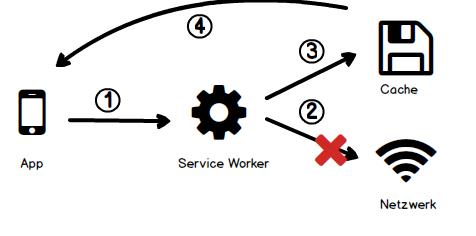
\includegraphics[width=0.75\textwidth]{networkfirst.png}
	\caption{\enquote{Erst Netzwerk, dann Cache}}
	\label{fig:cachingNetworkFirst}
\end{figure}



\subsubsection{\enquote{Erst Cache, dann Netzwerk}}
Wie Abbildung \ref{fig:cachingCacheFirst} zeigt, wird der Request hier zuerst an den Cache weitergeleitet. Befindet sich die angefragte Datei nicht im Cache, wird die Anfrage als \ac{HTTP}-Request an den Server weitergeleitet. Dies ist die bevorzugte Strategie für die meisten Requests in Offline-First Anwendungen.\autocite[Kapitel 05]{BookBuildingPWAs}.

\begin{figure}[h]
	\centering
	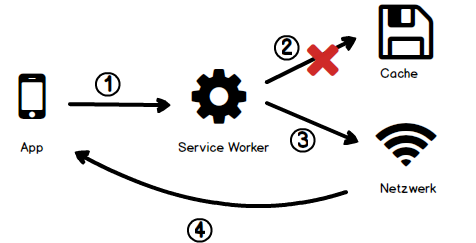
\includegraphics[width=0.75\textwidth]{cachefirst.png}
	\caption{\enquote{Erst Cache, dann Netzwerk}}
	\label{fig:cachingCacheFirst}
\end{figure}

\subsubsection{\enquote{Nur Netzwerk}}
Für Aufgaben, die nur Online zu erfüllen sind, eignet sich die in Abbildung \ref{fig:cachingNetworkOnly} bezeichnete Strategie. Hier leitet der Service Worker den Request nur an das Netzwerk und nie an den Cache weiter. Offline-First Applikationen sollten so konzipiert sein, dass diese Art Requests im Falle einer unterbrochenen Internetverbindung nachgeholt werden können, wenn der Nutzer wieder online ist.

\begin{figure}[h]
	\centering
	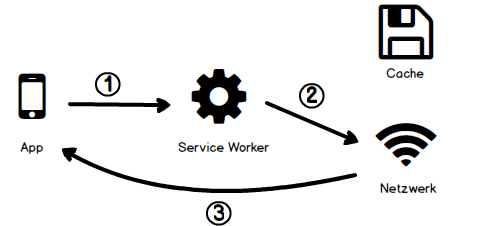
\includegraphics[width=0.75\textwidth]{networkonly.png}
	\caption{\enquote{Nur Netzwerk}}
	\label{fig:cachingNetworkOnly}
\end{figure}

\subsubsection{\enquote{Nur Cache}}
Abbildung \ref{fig:cachingCacheOnly} zeigt, wie die angefragte Ressource nur im Cache abgefragt wird. Diese Strategie ist nur dann sinnvoll, wenn die betroffenen Daten in einem vorherigen Schritt, beispielsweise beim Installieren des Service Workers, mit gecached wurden.

\begin{figure}[h]
	\centering
	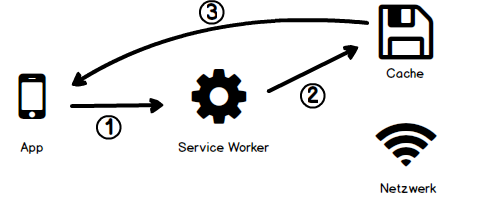
\includegraphics[width=0.75\textwidth]{cacheonly.png}
	\caption{\enquote{Nur Cache}}
	\label{fig:cachingCacheOnly}
\end{figure}

\section{Offline First Applikationen als verteilte Systeme}\label{sec:OfflineFirstVerteiteSysteme}
\citet{ArticleDistributedSystems} beschreiben verteilte Systeme wie folgt: \enquote{Ein verteiltes System ist eine Sammlung von autonomen Rechenelementen, die den Benutzern als ein einziges kohärentes System erscheint.}

Die folgende Liste zeigt die Charakteristika von verteilten Systemen, zusammengefasst nach \citet{BookDistributedSystemsDefinition}.

\begin{description}
\item[Eigenständige Computer] In einem verteilten System sind mehrere eigenständige Computer zu einem System verbunden. Diese können sich sowohl in der Hardware, als auch in der Funktionsweise unterscheiden. 
\item[Singuläres Erscheinungsbild] Für den Nutzer sind die Unterschiede zwischen den einzelnen Computern im System unersichtlich. Er nimmt die verteilten Computer als ein einzelnes System wahr. 
\item[Konsistente und einheitliche Interaktion]
	Eine Konsequenz aus dem singulären Erscheinen bedeutet, dass die Interaktion des Nutzers mit dem System immer gleich sein sollte, unabhängig davon, mit welcher Schnittstelle des Systems er tatsächlich interagiert. 
\item[Kontinuierliche Verfügbarkeit]
	Das System soll dem Nutzer kontinuierlich zur Verfügung stehen, auch wenn einzelne Teile des Systems vorübergehend ausgefallen oder nicht erreichbar sind.
\end{description}
\label{tab:charakteristikaDistributedSystem}

%TODO satz einfügen Kleppnmann vortrag.
Die folgende Liste zeigt, dass funktionsfähige Offline-First Applikationen die gleichen Charakteristika aufweisen und fasst zusammen, welche Rolle diese Merkmale in der Applikation spielen.

\begin{description}		
\item[Eigenständige Computer] Der Server und verschiedene Endgeräte bilden ein System. Sobald ein Endgerät die Applikation zwischenspeichert, ist sie als eigenständiger Computer im System aktiv. Als Endgerät qualifiziert sich jedes Gerät, welches einen kompatiblen Browser betreibt, weshalb die Endgeräte auch untereinander über unterschiedlichste Hardware verfügen können.
\item[Singuläres Erscheinungsbild]Die Kernfunktionalität von Offline-First Applikationen ist die Offlinefunktionalität. Offline interagiert der Nutzer nur mit seinem Endgerät, online werden die Daten gleich an den Server geschickt. Diese Unterschiede sind für den Nutzer jedoch nicht von Belang. \item[Konsistente und einheitliche Interaktion]
Unabhängig davon, welches Endgerät der Nutzer verwendet, sollen ihm früher oder später die Änderungen aller im System aktiven Geräte angezeigt werden. Der Nutzer muss sich zu keinem Zeitpunkt Gedanken darüber machen, aus welchen Computern das System besteht.
\item[Kontinuierliche Verfügbarkeit]
Ein weiterer Aspekt, welcher sich aus der verbindlichen Offlinefunktionalität ergibt, ist die kontinuierliche Verfügbarkeit. Der Nutzer kann seine Arbeit auch fortführen, wenn der Server nicht erreichbar ist. Durch SEC landen diese Änderungen früher oder später im System, wodurch die getrennte Verbindung zum Server keine Auswirkungen auf dessen Funktionsumfang hat. 
\end{description}
\label{tab:charakteristikaOfflineFirst}

Daraus ergibt sich, dass es sich bei Offline-First Webanwendungen um verteilte Systeme handelt. Diese Erkenntnis kann dabei helfen, Probleme von Offline-First Applikationen zu lösen. Bei Offline-First handelt es sich um ein relativ junges Konzept. Obwohl Progressive Web Apps mittlerweile häufig im Netz anzutreffen sind, erfüllt deren Offlinefunktionalität selten Offline-First Kriterien. Für Probleme wie die in Abschnitt \ref{sec:Problemfeld} beschriebene Synchronisation von Daten gibt es deshalb wenige beschriebene Lösungsansätze oder konkrete wissenschaftliche Arbeiten (siehe \ref{sec:VerwandteArbeiten}). Mit verteilten Systemen hingegen beschäftigt sich die Informatik bereits seit den 70er Jahren \autocite{Andrews1999FoundationsOM}. Lösungen, welche für die Herausforderungen von verteilten Systemen entwickelt wurden, kommen also auch für Offline-First Webapplikationen in Frage. Eine dieser Lösungen ist die Nutzung von optimistischen Replikationsverfahren. 

\section{Replikation}

Eine der wichtigsten Grundlagen verteilter Systeme ist die Replikation von Daten. Datenreplikation beschreibt das Verwalten mehrerer Datenspeicher, genannt Replikationen. Diese Replikationen halten die gleichen Daten, befinden sich jedoch auf unterschiedlichen Computern \autocite[S.42]{ArticleOptimisticReplication}. \citet{BookDistributedSystemsConceptsAndDesign} nennen drei Aspekte, zu denen Replikation in verteilten Systemen entscheidend beiträgt: Performancesteigerung, erhöhte Verfügbarkeit und Fehlertoleranz. Somit trägt diese Technik entscheidend dazu bei, sowohl kontinuierliche Verfügbarkeit als auch konsistente Interaktion, beschrieben in \ref{tab:charakteristikaDistributedSystem}, zu garantieren. Vom aus dem Netz nicht mehr wegzudenkenden Caching bis hin zu aufwendigeren Aufgaben wie Load-Balancing oder der Verarbeitung von DNS-Requests bietet das Internet zahlreiche Anwendungsfelder, in denen Replikation angewendet wird. 

\subsection{Pessimistische Replikation: Strong Consistency}

Traditionelle Strategien, um die Replikationen auf dem selben Stand zu halten folgen dem Modell der \ac{SC}. \ac{SC} setzt voraus, dass alle Replikationen stets identisch sind, als gäbe es konstant nur eine singuläre Kopie der Daten. Wenn ein Update auf einer Replikation erfolgt, muss es direkt auf allen weiteren Replikationen übernommen werden. 

Es gibt ein weites Spektrum an Lösungen, um \ac{SC} zu gewährleisten.Diese reichen von {Update=-Everywhere} Systemen, die einzelne Änderungen sofort auf allen Replikationen speichern \autocite{ThesisUpdateEverywhere} bis zu \enquote{primary copy} Lösungen \autocite[S.14]{BookPrimaryReplica}, welche Änderungen von einem primären Datenspeicher auf alle weiteren Replikationen verteilen. Gemeinsam haben diese Algorithmen die Tatsache, dass sie keinen Zugriff auf Replikationen gewähren, welche nicht auf dem aktuellsten Stand sind \autocite[S.43]{ArticleOptimisticReplication}. Für Offline-First Anwendungen kommt diese Art der Replikation nicht in Frage. Die Anforderung, dass die Verbindung zum Netzwerk stets unterbrochen sein kann (siehe \ref{sec:DefinitionOfflineFirst}), ist mit diesem Prinzip nicht vereinbar. Sobald eine Replikation vom Netzwerk getrennt ist, ist es unmöglich zu garantieren, dass sie auf dem aktuellsten Stand ist.

\subsection{Optimistische Replikation: Eventual Consistency}

Die optimistische Replikation, auch genannt \acf{EC}, ist ein alternatives Modell der Datenreplikation, welches den Replikationen erlaubt, voneinander abzuweichen.

Die Implementierung von optimistischer Replikation bietet sich somit als Lösung für Systeme an, welche besonderen Wert auf kontinuierliche Verfügbarkeit legen, wie Offline-First Applikationen (siehe Sektion \ref{sec:OfflineFirstVerteiteSysteme}). 

Bei der Verwendung von optimistischer Replikation sind Änderungen an Replikationen jederzeit gestattet, auch wenn diese nicht auf dem aktuellsten Stand sind, oder keine Verbindung zum Netzwerk haben. Nimmt der Nutzer eine Änderung vor, so wird diese auf seiner Replikation sofort umgesetzt. Im Hintergrund wartet die Applikation nun darauf, diese Änderung an die restlichen Computer des verteilten Systems weiterzugeben sowie selbst Änderungen entgegenzunehmen und zu verarbeiten \autocite[S.46]{ArticleOptimisticReplication}. Ziel ist es, wie beim Modell der Strong Consistency, Einheitlichkeit unter den Replikationen herzustellen. Das Modell der \ac{EC} setzt jedoch nicht voraus, dass diese Einheitlichkeit sofort erfolgen muss, sondern nur zu einem beliebigen späteren Zeitpunkt. 

Da die Computer im System parallel Änderungen vornehmen können, kann es vorkommen, dass mehrere Replikationen das gleiche Datenobjekt modifizieren. Im Allgemeinen werden die Modifikationen zu unterschiedlichen Ergebnissen führen. Ist dies der Fall, spricht man von einem Konflikt. Das Ziel, Konvergenz zwischen den Replikationen zu erlangen, kann nur erreicht werden, wenn aus allen im Konflikt stehenden Änderungen eine einheitliche Lösung entsteht.

Deshalb muss ein System, welches \ac{EC} implementiert, die Funktionalität aufweisen, Konflikte zu beheben. Problematisch dabei ist, dass die Replikationen nicht auf dem gleichen Stand sind bis der Konflikt vollständig behoben ist, selbst nachdem sie ihre Änderungen untereinander ausgetauscht haben. Der Prozess der Konfliktbehandlung kann voraussetzen auf die manuelle Konfliktlösung von Nutzern oder die Daten anderer Replikationen zu warten. \autocite{ArticleEventualConsistencyConflicts}

Gerade in Offline-First Anwendungen ist die Konfliktbehandlung eine große Herausforderung, wie in Abschnitt \ref{sec:Problemfeld} ausgeführt wird. Um diese Herausforderung zu bewältigen, bietet das Modell der \acf{SEC} einen Ansatz, die Flexibilität von \ac{EC} mit der Sicherheit von \ac{SC} zu erweitern. 



%TODO: Nachteile Eventual Consistency:
%- Conflict Resolution
%- Garantiert nur, dass alle Updates ankommen. Dies kann zu Konflikten führen (Node A schreibt X=2, Node B schreibt X=3. Also ist erst A dann B = 3, erst B dann A = 2). Kann behoben werden durch Conflict Resolution, aber die ist stressig. 
%- Überleitung zu SEC. In SEC kommen alle Updates in der gleichen Reihenfolge, so kann komplexe Conflict Resolution umgangen Werden. 

\subsection{Strong Eventual Consistency}

%TODO Auf dem gleichen Stand = Konvergent/Konvergenz austauschen

\ac{SEC} beschreibt eine spezielle Form der \acf{EC}, welche das System von der Last der Konfliktbehandlung bereit. \ac{SEC} garantiert, dass zwei Replikationen nach dem Austauschen ihrer Änderungen immer konvergent sind. Im Gegensatz zur \ac{EC} wird die Konfliktbehandlung nicht vom System übernommen, stattdessen wird dieser Prozess durch die Nutzung spezieller Datentypen überfällig.

%TODO Abbildungen zu Consistencies
%TODO Evtl Charakteristika beschreiben 

\section{CRDTs}

CRDTs sind abstrakte Datentypen, die in verteilten Systemen eingesetzt werden um \ac{SEC} zu ermöglichen. Sie basieren auf klassischen Datentypen wie Registern, Sets und Maps. CRDTs erweitern diese Datentypen um eine Schnittstelle, welche das Daten-Objekt neben den klassischen Operationen wie dem Auslesen des gespeicherten Wertes um Funktionalitäten erweitert um \ac{SEC} zu gewährleisten.\autocite[S.1 ]{ArticleCRDTOverview}

Der Satz an CRDT-Funktionalitäten enthält immer eine Funktion zum aktualisieren des Wertes des Objekts. Weitere Daten, um welche CRDTs klassische Datentypen erweitern, lassen sich als Metadaten beschreiben. Ihr Zweck ist es, die aktualisierungs-Funktionalität möglich zu machen. Soll ein CRDT-Objekt beispielsweise so aktualisiert werden, dass sich die neuste Änderung des Wertes immer gegen ältere durchsetzt, muss zusätzlich zum Wert noch ein Zeitstempel der letzten Änderung verwaltet werden (siehe \ref{sec:LWW REGISTER}).
%todo WERT = Besseres wort finden? Value?
%todo: Abbildung CRDT mit Value, Merge, Zusatz
Die Datentypen werden speziell so modelliert, dass das aktualisieren von CRDTs kommutativ, assoziativ und idempotent erfolgen kann \autocite{InproceedingsCrdtsInProduction}.

\begin{description}
	\item[Kommutativ] Wenn zwei CRDTs Aktualisierungen austauschen, ist das Ergebnis identisch, unabhängig davon, in welcher Reihenfolge dies geschieht (a merge b == b merge a)
	\item[Assoziativ] Wenn drei CRDTs nacheinander zusammengeführt werden, ist das Ergebnis immer gleich, unabhängig davon welche zwei der Objekte zuerst Aktualisierungen austauschen. (a merge (b merge c) == b merge (a merge c))
	\item[Indempotent] Das einmalige zusammenführen zweier CRDTs hat das gleiche Ergebnis wie ein beliebig oftes Wiederholen des Vorgangs. (a merge b = ((((a merge b)merge b)merge b)merge b))
\end{description}

Diese Eigenschaften führen dazu, dass zwei Replikationen deterministisch im gleichen Zustand befinden müssen, sobald sie den Stand ihrer Daten synchronisiert haben. Im Gegensatz zur \ac{EC} ist das System nicht mehr von einer im Konsens zu geschehenden Konfliktlösung abhängig. 

Dieser Vorteil von \ac{SEC} ist gleichzeitig der größte Nachteil bei der Nutzung von CRDTs in der Praxis. Nicht alle Datenstrukturen lassen sich so modellieren, dass sie die benötigten oben genannten Anforderungen erfüllen. Zwar gibt es bereits viele, gut dokumentierte, kompatible Datentypen (siehe \ref{sec:Verwandte Arbeiten}), dennoch bedarf die Verwendung von CRDTs und \ac{SEC} ausgiebiger Planung und ist in manchen Fällen schlichtweg nicht möglich. 

In der Literatur werden CRDTs in state-based und operation-based unterteilt \autocite[S. 10]{ArticleOptimisticReplication}. Die Unterscheidung Erfolgt danach, das Zusammenführen der Objekte funktioniert.

\begin{description}
	\item[State-based]
	Beim Synchronisieren von state-based CRDTs, wird der gesamte State der Objekte ausgetauscht.
	Die merge Funktion ist anschließend in der Lage, beide Stati zu einem zu kombinieren. 
	
	\item[Operation-based]
	Bei der Variante der operation-based CRDTs wird nicht der gesamte State der Objekte ausgetauscht. Stattdessen erfolgt der Austausch über einzelne Updates. Wird der State eines Objektes geändert, so wird die Operation, welche die Änderung hervorgerufen hat, gespeichert. Beim mergen zweier Objekte, werden diese Updates ausgetauscht und anschließend auf das jeweils andere Objekt angewandt. Da die Operationen kommutativ sein müssen,
	%todo Siehe oben?
	ist die Reihenfolge der Updates nicht relevant. 
\end{description} 

Beide Kategorien sind equivalent\autocite[S. 9]{InproceedingsCRDTOriginal}, was bedeutet das ein state-based CRDT ein operation-based CRDT emulieren kann und vice versa.

%todo hier ein paar beispiele oder so ka

\subsection{LWW-Register}
Ein Register ist ein Objekt welches einen einzelnen Wert verwaltet. Dieser Wert kann jede vom System unterstützte Datenstruktur sein. Ein \ac{LWW-Register} verfügt neben dem Wert noch über einen Zeitstempel. Wird der Wert des Registers geändert, wird auch der Zeitstempel auf den Zeitpunkt dieser Änderung gesetzt. Beim Zusammenführen zweier Register kann so immer die neuste Änderung übernommen werden. Da sowohl Wert als auch Zeitstempel ausgetauscht werden, handelt es sich hier um ein state-based CRDT.

%TODO Counter auslassen weil ich ihn nicht benutze?
\subsection{Grow-Only Set}
Ein Set ist eine Datenstruktur, welche eine Sammlung von Objekten verwaltet. Traditionelle Operationen eines Sets umfassen das Hinzufügen und Entfernen von Objekten. Diese Operationen sind nicht jedoch kommutativ: Wird dem Set ein Objekt erst hinzugefügt und anschließend entfernt, ist es im Endeffekt nicht mehr im Set vorhanden. Wird es jedoch erst entfernt und anschließend hinzugefügt, so existiert das Objekt daraufhin weiterhin im Set.

Ein Grow-Only Set löst dieses Problem durch das Auslassen der Entfernen Operation. Das Entfernen des Objektes kann durch einen \enquote{Tombstone} Wert ersetzt werden. Ist dieser Wert positiv, wird der Eintrag vom System so behandelt, als wäre er nicht vorhanden. Somit ist das Set wieder kommutativ, und die Funktionalität des Löschens bleibt bestehen. 

%todo OPERATIONEN KURSIV? IRGENDWIE HERVORHEBEN

\section{Hybrid-Logical Clocks}

\chapter{Konzeption}
\section{Anforderungsanalyse}

In diesem Kapitel werden die funktionalen und nicht funktionalen Anforderungen an den im Rahmen dieser Arbeit entwickelten Prototypen beschrieben.

\subsection{Funktionale Anforderungen}
Zweck der funktionalen Anforderungen ist es, Verhalten und Funktionalität zu entwickelnden Systems zu beschreiben. Die formulierten Anforderungen sollen somit einen Überblick darauf geben, was das implementierte System erfüllen muss. Da das Ziel dieser Arbeit die Entwicklung einer Datenstruktur für eine Offline-First Applikation ist (siehe \ref{sec:Einleitung}), liegt der Fokus der gesammelten Anforderungen eindeutig auf dem Zusammenspiel zwischen Offline-First und CRDTs.

Üblich in einer Anforderungsanalyse ist, die Anforderungen in \enquote{kann}, \enquote{soll} und \enquote{muss} Kategorien einzuteilen. Da es sich hier um die Entwicklung eines Prototypen handelt, wird sich in diesem Teil exklusiv auf \enquote{muss} Anforderungen beschränkt. Hierbei handelt es sich um Anforderungen, welche essentiell für das System sind.

\begin{description}
	\item[{[]} Anlegen von Zutaten]
	Der Nutzer soll in der Lage sein, Zutaten zu einem Rezept hinzuzufügen.
	\item[{[]} Zugriff mit mehreren Endgeräten gleichzeitig]
	Der Nutzer soll in der Lage sein, mit mehreren Geräten gleichzeitig auf das gleiche Rezept zuzugreifen.
	\item[{[F01]} Offline-Erreichbarkeit]
	Der Nutzer der Anwendung muss in der Lage sein, die Anwendung offline nutzen zu können
	\item[{[F02]} Lokales Speichern]
	Die Anwendung muss über die Funktionalität verfügen, Änderungen von Nutzern lokal zu speichern, wenn keine Verbindung zum Netzwerk besteht.
	\item[{[F03]} Synchronisierung von Daten]
	Änderungen des Nutzers müssen mit dem Server synchronisiert werden können, wenn die Verbindung zum Netzwerk wiederhergestellt ist. Der Nutzer sollte niemals seine Arbeit verlieren.
	\item[{[]} Anlegen von Zutaten]
	Der Nutzer soll in der Lage sein, Zutaten zu einem Rezept hinzuzufügen.
	\item[{[]} Unabhängigkeit der Datenstruktur]
	Die implementierte Datenstruktur muss unabhängig von der benutzten Datenbank sein. Keine der umgesetzten CRDT-Funktionalitäten darf von der gewählten Datenbank abhängig sein. 
	\item[{[]} Abdeckung von Fehl]


\end{description}



\section{Software Architektur}
\section{User Interface}
\section{Schnittstellen}
\newpage
\printbibliography



\end{document}]


